%%%%%%%%%%%%%%%%%%%%%%%%%%%%%%%%%%%%%%%%%%%%%%%%%%%%%%%%%%%%%%%%%
%        Contents: Bachelorarbeit, HS Fulda        %
%                          31.08.2022                        %
%---------------------------------------------------------%
%                         Evaluation.tex                     %
%                        by Carina Möller                   %
%                    cary_moeller@gmx.de              %
%%%%%%%%%%%%%%%%%%%%%%%%%%%%%%%%%%%%%%%%%%%%%%%%%%%%%%%%%%%%%%%%%

\chapter{Evaluation} \label{EV}

%  Das Kapitel noch gescheiter ausbauen... mögliche Evaluationsmethoden:
%  - Abhaken der Ziele?
%  - ExpertenUmfragen?
%  - Benchmarks?

Das Ziel dieser Arbeit ist es, verschiedene Prototypen für die Transformationsengine zu implementieren, um daraufhin denjenigen Ansatz zu identifizieren, der am Besten für die Einbindung in die \xblackout{UDI Platform} geeignet ist.\\
Im folgenden Kapitel werden daher die vorgestellten Lösungsansätze analysiert und miteinander verglichen. Die Grundlinie stellt dabei die spezifische Version aus Kapitel\nbs\ref{HC} dar\nbs --\nbs ihr gegenüber stehen die generischen Ansätze aus Kapitel\nbs\ref{ED} und\nbs\ref{MD}. Unabhängig davon wird zusätzlich die Wahl der JSON"=Abfragesprache evaluiert und abschließend auf die Eignung der Transformationsengine für den Massen"=Upload eingegangen.


\section{Gegenüberstellung der drei Ansätze}\label{G3A}

Die Evaluation untersucht den Nutzen bzw. die Eignung der Transformationsengine"=Varianten, indem die verschiedenen Ansätze anhand Kriterien bzgl. Funktionalität und Benutzerfreundlichkeit empirisch bewertet werden, mit dem Zweck sie zu vergleichen, um die beste Lösung für die \xblackout{UDI Platform} zu finden. Näheres zu Evaluationen beschreiben\nbs\cite{eval:sta} und\nbs\cite{eval:meth}.

Die drei Varianten der Transformationsengine werden mit dem Kapitel, in dem ihr Konzept vorgestellt wurde, nummeriert. Es wird also der spezifische Ansatz\nbs\ref{HC} sowie die generischen Versionen, Ansatz\nbs\ref{ED} mit der Abbildung in der Excel"=Datei und Ansatz\nbs\ref{MD} mit der zusätzlichen Mapping"=Datei, evaluiert.\\
Die Kriterien basieren auf den funktionalen und nicht-funktionalen Anforderung an die Transformationsengine, welche in Tabelle\nbs\ref{tab:fnfa} spezifiziert wurden, wobei bzgl. der Benutzerfreundlichkeit\nbs\ref{anf:bf} noch differenzierter unterteilt wird. In einem Soll/Ist"=Vergleich wird die Erfüllung der Ziele überprüft.\\
Zur Bewertung wird ein einfaches Ampelsystem mit den Stufen
\begin{itemize}[leftmargin=7em]
\item[Gut \,\bgood] Kriterium in vollem Maße / gut erfüllt 
\item[Mittel \,\bokay] Kriterium teilweise / rudimentär erfüllt 
\item[Schlecht \,\bbad] Kriterium nicht / schlecht erfüllt
\end{itemize}
verwendet, wenngleich einige Kriterien nur \bgood[4pt] oder \bbad[4pt] zulassen.

Insgesamt ergibt sich die folgende Evaluationsmatrix:

\begin{table}[htbp]
\centering
\begin{tabular}[h]{|l|l|M{0.7cm}|M{0.7cm}|M{0.7cm}|}
\hline
\multirow{2}{*}{\,Nr.} & \multirow{2}{*}{Kriterium} & \multicolumn{3}{c|}{Ansatz}\Tstrut\\
& & \ref{HC} & \ref{ED} & \ref{MD}\Bstrut\\
\hhline{=====}
\,\ref{anf:trans} & Datentransformation nach Excel & \good & \good & \good\Tstrut\\
\,\ref{anf:bool} & Mapping von Wahrheitswerten & \good & \good & \good\\
\,\ref{anf:date} & Mapping von Datumsformaten & \good & \bad & \good\\
\,\ref{anf:elem} & Mapping von Element-Wertelisten\, & \good & \good & \good\Bstrut\\
\arrayrulecolor{mygrey1}\hline\arrayrulecolor{black}
\,\ref{anf:gen} & Aufwand bei Änderung/Erweiterung & \bad & \good & \good\Tstrut\\
\,\ref{anf:bf}.1\, & Übersichtlichkeit für Benutzer & \bad & \okay & \good\\
\,\ref{anf:bf}.2\, & Fehleranfälligkeit für Benutzer & \bad & \good & \okay\\
\,\ref{anf:mu} & Massen-Upload möglich  & \good & \good & \good\Bstrut\\
\hline
\end{tabular}
\caption{\label{tab:eval1}Evaluationsmatrix für die Transformationsengine}
\end{table}
Da Ansatz 3.2 lediglich skizziert anstatt in der Praxis implementiert wurde, werden die Kriterien bzgl. ihrer Machbarkeit aus theoretischer Sicht bewertet. Außerdem ist anzumerken, dass das Mapping für Datumsangaben in Ansatz\nbs\ref{ED} nur aus Zeitgründen eingespart wurde, aber durchaus realisiert werden kann.
Im Folgenden wird die obige Bewertung noch genauer erläutert. Auf den Massen-Upload wird gesondert in Abschnitt\nbs\ref{MUT} eingegangen\nbs --\nbs die verschiedenen Ansätze unterscheiden sich diesbezüglich nicht, da er vor allem von der Verwendung der Excel"=Bibliothek abhängig ist. 

\enlargethispage{\baselineskip}
Der spezifische \fe{Ansatz\nbs\ref{HC}}, welcher auf Hartkodierung setzt, hat den Vorteil, dass die Implementierung absolut unkompliziert ist. Die einzige Herausforderung ist der richtige Umgang mit der Excel"=Bibliothek \bib{Apache POI}.\\
Hier wirkt sich allerdings jede kleine Änderung direkt aus. Nicht nur bei neuen Behörden muss das Package erweitert werden, sondern es ergeben sich auch Codeänderungen, sobald eine Behörde ihre Anforderungen und damit ihre Vorlage minimal abändert. Ebenso wenn intern bzw. beim Hersteller Datenelemente überarbeitet werden. Aufgrund der Hartkodierung müssen Änderungen oder Erweiterungen jedes Mal manuell eingepflegt und ausgerollt werden. Die stets neuen Versionen und ihr Deployment führen zu erheblichem Aufwand, zumindest wenn auf regulatorischer Seite häufiger Anpassungen auftreten bzw. die Plattform kontinuierlich durch neue Märkte erweitert wird. 

Daher werden stattdessen \fe{generische Ansätze} zur Lösung angestrebt, die unabhängig von Behörden, Herstellern und Produktinformationen sind. Hier muss bei einer externen oder internen Änderung durch die Behörde oder \xblackout{p36} lediglich die neue (in Ansatz\nbs\ref{ED} überarbeitete) Excel"=Vorlage im System hinterlegt und in Ansatz\nbs\ref{MD} außerdem die gespeicherte YAML"=Datei aktualisiert werden. Dabei ist entscheidend, dass für diese Änderungen keine speziellen, tiefergehenden Programmierkenntnisse nötig sind, sondern dass auch jemand mit nur oberflächlichem Wissen die Umsetzung ausführen, d.\,h. die Transformationsengine bedienen, kann. Ansatz\nbs\ref{HC} bietet hingegeben keine Benutzung in diesem Sinn.

Der Vorteil von \fe{Ansatz\nbs\ref{ED}}, bei dem man die Abbildung in den jeweiligen Excel"=Arbeitsblättern verankert, besteht darin, dass nur eine einzige zusätzliche Datei nötig ist und der Nutzer visuell genau vor Augen hat, welche Daten in welche Spalten geschrieben werden. Beim Erstellen des Mappings müssen also nicht zwei Dateien miteinander abgeglichen werden, wodurch Tippfehler minimiert werden. Ein Nachteil ist allerdings, dass die Bearbeitung von Excel"=Dateien unbequem ist und insbesondere längere Ausdrücke bei der JSON"=Abfrage in den Excel"=Zellen nicht mehr leserlich dargestellt werden können. 

\fe{Ansatz\nbs\ref{MD}} geht einen kleinen Umweg über eine zusätzliche Datei zur Beschreibung des Mappings. Im YAML"=Format ist sie besonders schlicht, schlank und übersichtlich. Während man die \bib{JSONata}"=Ausdrücke auf den ersten Blick in voller Gänze lesen kann und auch mehrzeilige Funktionen unterstützt werden, muss natürlich die Abbildung als solche zunächst definiert werden. Das heißt, die Namen aller Tabellenblätter, die jeweiligen Startreihen, sowie die Spalten und ihr gewünschter Inhalt müssen abgetippt bzw. angegeben werden. Das bringt einen gewissen Aufwand und Fehleranfälligkeit mit sich. Zusätzliche Flexibilität und Struktur erhält man durch die unkomplizierte Definition von Mappings für Wahrheitswerte, Datumsformate oder einzelne Datenelemente. Die YAML"=Datei kann hierbei auf umkomplizierte Weise beliebig erweitert werden, falls neue Funktionen implementiert werden\nbs --\nbs zum Beispiel die Angabe einer Maximalanzahl an Zeilen. Ist der Maximalwert erreicht, werden alle weiteren Produkte in eine neue Arbeitsmappe geschrieben, um Overflow zu vermeiden.

\enlargethispage{\baselineskip}
Insgesamt kristallisiert sich der letzte Ansatz als der Beste heraus. Die gewonnene Übersicht durch die klare und intuitive Struktur der YAML"=Datei rechtfertigt die zusätzliche Datei und mögliche Übertragungsfehler. Für die \xblackout{UDI Platform} wird daher Ansatz\nbs\ref{MD} empfohlen. 

\section{JSON-Abfragesprache}\label{JAS}

Neben der bereits angesprochenen Unterscheidung, wo und wie die Mapping Informationen gespeichert werden, also konkret in welcher Datei, ist auch die Wahl der Abfragesprache von Bedeutung. Sie legt zu einem gewissen Teil Form und Umfang der Abbildung zwischen der Excel"=Vorlage und den Produktdaten fest. Einen detaillierten Überblick über eine Auswahl verschiedener JSON"=Abfragesprachen und ihrer Eigenschaften bzw. Vor"~ und Nachteile vermittelt das Grundlagenkapitel\nbs\ref{JQL}. \\
Als Einstieg in die Thematik wurde anfänglich \bib{JSONPath} verwendet, wobei sich schnell die ersten Grenzen aufgezeigt haben. Daher wurde in Ansatz\nbs\ref{ED} zunächst auf \bib{JMESPath} gesetzt und später in Ansatz\nbs\ref{MD} auf \bib{JSONata} umgestellt. Die JSON"=Abfragesprachen sind unabhängig von den vorgestellten Ansätzen und entsprechend beliebig kombinierbar: Variante\nbs\ref{ED} mit \bib{JSONata}"~ anstatt \bib{JMESPath}"=Ausdrücken im Excel"=Arbeitsblatt wäre z.\,B. genauso möglich.

Die Kriterien für die Evaluation, um die für \xblackout{p36} am besten geeignete Abfragesprache zu ermitteln, betreffen zum einen die Sprache selbst und zum anderen deren Anwendung innerhalb der Transformationsengine. 
Es wird die Mächtigkeit der Sprache begutachtet\nbs --\nbs im konkreten Fall heißt das, ob mit ihr die Werte der Datenelemente in die typischerweise von den Behörden gewünschte Form transformiert werden können und darüber hinaus ggf. noch komplexere Abfragen möglich wären. Daneben wird die Erweiterbarkeit durch selbst definierte Funktionen beurteilt, und wie übersichtlich und intuitiv die Syntax ist, sowie das Verhalten im Anwendungsfall bei komplexen Datenelementen. Die vorhandenen Java"=Implementierungen werden bzgl. Umfang, Verbreitung und Aktualität beurteilt. Außerdem wird der Aufwand gemessen, den die Benutzer zur Einarbeitung in bzw. im Umgang mit der Sprache haben.

\enlargethispage{\baselineskip}
Unter Verwendung des Ampelsystems aus Abschnitt\nbs\ref{G3A} ergibt sich die folgende Evaluationsmatrix, deren Einträge im Nachgang noch genauer erläutert werden.

\begin{table}[htbp]
\centering
\begin{tabular}[h]{|l|c|c|c|}
\hline
Kriterium & JSONPath & JMESPath & JSONata \TBstrut\\
\hhline{====}
Mächtigkeit & \bad & \okay & \good\Tstrut\\
Erweiterbarkeit & \okay & \good & \good\\
Übersichtlichkeit der Syntax & \good & \okay & \good\\
Abfrage komplexer Elemente & \good & \okay & \okay\\
Java"=Bibliothek & \good & \good & \okay\\
Einarbeitungsaufwand & \okay & \bad & \good\Bstrut\\
\hline
\end{tabular}
\caption{\label{tab:eval1}Evaluationsmatrix für die JSON-Abfragesprache}
\end{table}

\bib{JSONPath} ist weit verbreitet, sehr populär und dient sicher als erste Anlaufstelle. Im Vergleich ist es allerdings auch die simpelste und am wenigsten mächtigste Abfragesprache von den hier verwendeten. Die Implementierung von \bib{JSONPath} in Java durch Jayway bietet über die reine Spezifikation hinaus Zusatzfunktionalitäten, wie z.\,B. einige eingebaute Funktionen und diverse Filtermöglichkeiten, siehe\nbs\cite{jayway}. Komplexere Funktionen, wie zum Beispiel den ternären Operator oder \texttt{contains} zur Abfrage von Array"=Inhalten, werden allerdings nicht unterstützt und können auch nicht innerhalb der Abfrage selbst definiert werden, sondern nur in der Implementierung der Engine. Es gibt hier den großen Vorteil, dass mit der Konfigurationsoption \texttt{DEFAULT\_PATH\_LEAF\_TO\_NULL} automatisch Nullwerte für fehlende Pfade bzw. Blätter zurückgegeben werden, was bei den relationalen Arbeitsblättern wichtig ist. Wie bereits in Kapitel\nbs\ref{IED} und\nbs\ref{IMD} angesprochen, muss hierfür sowohl bei \bib{JMESPath} als auch \bib{JSONata} auf einen Workaround zur absichtlichen Erzeugung von Nullwerten gesetzt werden, der die Ausdrücke etwas aufbläht.

Die Abfragesprache \bib{JMESPath} besticht besonders durch den im Vergleich zu \bib{JSONPath} deutlich angestiegen Umfang und ihre ausführliche Dokumentation, auch wenn die Sprache in ihrer Komplexität zugenommen hat. Mit der Hintereinanderausführung per Pipe"=Symbol sind vielfältige Arraymanipulationen möglich, die zum Teil Arrays aufblähen und durch \texttt{[]} ggf. wieder abflachen, worunter die Übersichtlichkeit etwas leidet. Außerdem können eigene Funktionen definiert werden, wenn auch nicht in der Abfrage selbst. Insgesamt konnten mit \bib{JMESPath} aber alle bisher aufgetretenen Abfragen in der Transformationsengine realisiert werden. \bib{JMESPath} ist bestrebt in vielen Programmiersprachen als Schnittstelle zur Verfügung zu stehen, so auch in Java. Sie erfreut sich wachsender Popularität, wobei sie allerdings hinter \bib{JSONPath} zurückfällt.

\bib{JSONata} ist noch mächtiger, allerdings ohne dass die Syntax darunter leidet. Die Sprache hat den großen Vorteil, dass die Nutzer, das heißt die Mitarbeiter des \xblackout{Solution Management}, schon Erfahrung mit ihr gesammelt haben, da \bib{JSONata} bereits an anderer Stelle verwendet wird. Es ist also keine größere Einarbeitung oder Umstellung notwendig. Obwohl \bib{JSONata} ursprünglich nur für TypeScript und NodeJS entwickelt wurde, schafft die API \bib{JSONata4Java} Abhilfe, vgl.\nbs\cite{jsonata:java}. Die Bibliothek ist unscheinbar und hat vergleichsweise wenig Nutzer, wird jedoch kontinuierlich gepflegt. Vereinzelte Funktionen wurden bisher nicht implementiert, allerdings kommen sie in der Engine nicht zum Tragen, sodass es im vorliegenden Anwendungsfall kein wirklicher Nachteil ist. Dem gegenüber besteht hier ebenso die Möglichkeit, die Sprache durch eigene Funktionsdefinitionen zu erweitern, und zwar auch innerhalb des \bib{JSONata}"~Ausdrucks.

Insgesamt fällt die Wahl der Abfragesprache daher eindeutig auf \bib{JSONata}, deren Umfang und kompakte Schreibweise überzeugen, während sie die Benutzer nicht mit der Wissensaneignung einer zusätzlichen Sprache belastet.\\
Anzumerken ist, dass die Performanz der Sprachen bei der Betrachtung außer Acht gelassen wurde. Diese ist nicht ausschlaggebend für die Transformationsengine, da sie sich in jedem Fall im annehmbaren Bereich bewegt (wie im anschließenden Abschnitt erläutert wird), allerdings schneidet diesbezüglich \bib{JSONata} vermutlich weniger gut ab, vgl.\nbs\cite{eval:bm1} und\nbs\cite{eval:bm2}\footnote{In den Benchmarks werden die JavaScript"=Bibliotheken verglichen, nicht Java. Daher kann für den vorliegenden Fall keine konkrete Aussage bzgl. der Performanz getroffen werden.}. 
 

\section{Massen-Upload}\label{MUT}
Ein wichtiges Kriterium ist die Skalierbarkeit über der Anzahl der Produkte, die in die Excel"=Vorlage geschrieben werden sollen. Die Hersteller registrieren gerade beim Einstieg in einem neuen Markt bzw. als Neukunde von \xblackout{p36} nicht nur einzelne Produkte, sondern ihr gesamtes Portfolio. Hierzu muss die Transformationsengine in der Lage sein, Daten in der Größenordnung von 1.000 bis 10.000 Produkten zu übermitteln. Für noch größere Uploads besteht keine Anforderung, da man den Prozess ggf. auch wiederholt ausführen kann, im Folgenden werden allerdings die maximalen Grenzen ausgetestet.  

Dazu wurden beim finalen Ansatz\nbs\ref{MD} Modultests mit unterschiedlich vielen Produkten ausgeführt. Die Tests haben ergeben, dass bis zu 16.000 Mal das Beispielprodukt in die Vorlage geschrieben werden kann. Bei dem Versuch die Excel"=Datei mit 17.000 Produkten abzuspeichern, kommt es zum Heap"=Overflow und der OutOfMemoryError wird geworfen. Man muss hierbei bedenken, dass in den relationalen Arbeitsblättern für jedes Produkt nicht nur eine Zeile erzeugt wird, sondern mehrere. In den Tests wurde mit dem Faktor 10 gerechnet, das heißt ein Produkt erzeugt zehn Zeilen in der Excel"=Datei. \\
Zur Überprüfung, ob eine Arbeitsmappe erfolgreich ausgefüllt wurde, wird diese nach dem Schreiben erneut geladen, um so die Anzahl der Zeilen auszulesen. Hierbei ergeben sich schon früher Probleme. Ab 10.000 Produkten, das heißt also 100.000 Zeilen, konnte die Excel"=Datei nicht mehr über die Bibliothek \bib{Apache POI} eingelesen werden, sondern es kam zum Überlauf des Speichers und der OutOfMemoryError"=Ausnahme. Daher wurde ab dieser Größe ein Test schon als erfolgreich gezählt, wenn die Datei nur erzeugt wurde und existiert, ohne sie erneut zu öffnen und genauer zu untersuchen. Manuell ist das Öffnen natürlich ohne Probleme möglich und die Daten wurden auch korrekt gefüllt. 

\begin{figure}[htbp]
 \centering
 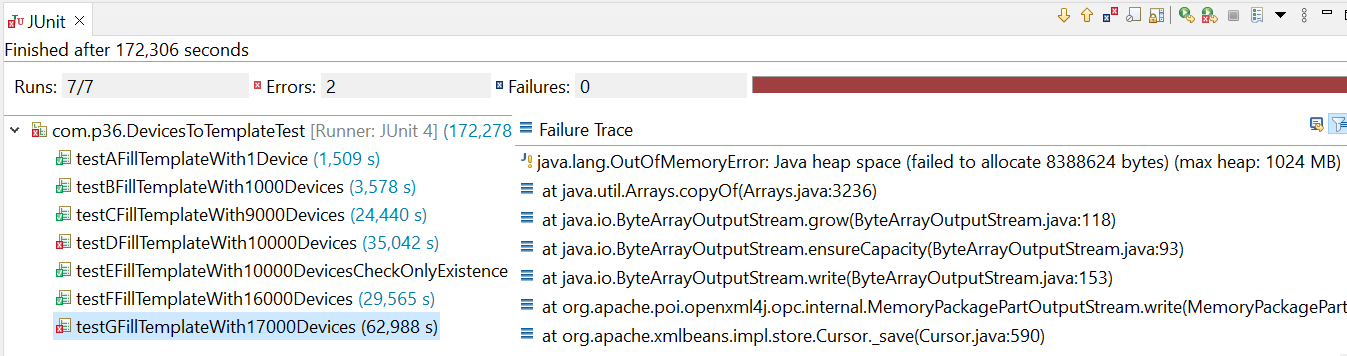
\includegraphics[width=\textwidth]{Bilder/MassUploadTests}
 \caption{Testergebnisse zum Massen-Upload}
 \label{fig:mu}
\end{figure}

Die Ergebnisse eines Testdurchlaufs sind in Abbildung\nbs\ref{fig:mu} festgehalten. Hier sieht man die Fehlermeldung bei 17.000 Devices. Auch im ersten Test mit 10.000 Devices, bei dem die Datei zur Überprüfung eingelesen wird, kommt es zu einem kleinen Heap"=Overflow. Die anderen Tests für bis zu 16.000 Produkten sind grün unterlegt und laufen erfolgreich durch. Der Massen"=Upload ist also mit der Transformationsengine realisierbar. Die Dauer des Schreibvorgangs bis zur erfolgreichen Excel"=Datei"=Erzeugung ist mit nur wenigen Sekunden sehr angenehm. Auch bei vielen Produkten bleibt die Zeit im Bereich von etwa 30 bis 60 Sekunden. Hierbei ist anzumerken, dass die Zeiten im Normalfall (wenn die Testreihenfolge nicht zur besseren Übersicht fixiert ist) stärker variieren, je nachdem welcher Test zuerst durchgeführt wird und damit ohne vorheriges Aufwärmen der JVM am längsten braucht. Trotz dieser Ungenauigkeiten verdeutlichen die Tests gut die Größenordnung der Geschwindigkeit des Transformationsprozesses. 




